% Options for packages loaded elsewhere
\PassOptionsToPackage{unicode}{hyperref}
\PassOptionsToPackage{hyphens}{url}
\PassOptionsToPackage{dvipsnames,svgnames,x11names}{xcolor}
\documentclass[
]{ltjsarticle}
\usepackage{xcolor}
\usepackage[margin=22mm]{geometry}
\usepackage{amsmath,amssymb}
\setcounter{secnumdepth}{-\maxdimen} % remove section numbering
\usepackage{iftex}
\ifPDFTeX
  \usepackage[T1]{fontenc}
  \usepackage[utf8]{inputenc}
  \usepackage{textcomp} % provide euro and other symbols
\else % if luatex or xetex
  \usepackage{unicode-math} % this also loads fontspec
  \defaultfontfeatures{Scale=MatchLowercase}
  \defaultfontfeatures[\rmfamily]{Ligatures=TeX,Scale=1}
\fi
\usepackage{lmodern}
\ifPDFTeX\else
  % xetex/luatex font selection
\fi
% Use upquote if available, for straight quotes in verbatim environments
\IfFileExists{upquote.sty}{\usepackage{upquote}}{}
\IfFileExists{microtype.sty}{% use microtype if available
  \usepackage[]{microtype}
  \UseMicrotypeSet[protrusion]{basicmath} % disable protrusion for tt fonts
}{}
\makeatletter
\@ifundefined{KOMAClassName}{% if non-KOMA class
  \IfFileExists{parskip.sty}{%
    \usepackage{parskip}
  }{% else
    \setlength{\parindent}{0pt}
    \setlength{\parskip}{6pt plus 2pt minus 1pt}}
}{% if KOMA class
  \KOMAoptions{parskip=half}}
\makeatother
\usepackage{longtable,booktabs,array}
\newcounter{none} % for unnumbered tables
\usepackage{calc} % for calculating minipage widths
% Correct order of tables after \paragraph or \subparagraph
\usepackage{etoolbox}
\makeatletter
\patchcmd\longtable{\par}{\if@noskipsec\mbox{}\fi\par}{}{}
\makeatother
% Allow footnotes in longtable head/foot
\IfFileExists{footnotehyper.sty}{\usepackage{footnotehyper}}{\usepackage{footnote}}
\makesavenoteenv{longtable}
\usepackage{graphicx}
\makeatletter
\newsavebox\pandoc@box
\newcommand*\pandocbounded[1]{% scales image to fit in text height/width
  \sbox\pandoc@box{#1}%
  \Gscale@div\@tempa{\textheight}{\dimexpr\ht\pandoc@box+\dp\pandoc@box\relax}%
  \Gscale@div\@tempb{\linewidth}{\wd\pandoc@box}%
  \ifdim\@tempb\p@<\@tempa\p@\let\@tempa\@tempb\fi% select the smaller of both
  \ifdim\@tempa\p@<\p@\scalebox{\@tempa}{\usebox\pandoc@box}%
  \else\usebox{\pandoc@box}%
  \fi%
}
% Set default figure placement to htbp
\def\fps@figure{htbp}
\makeatother
\setlength{\emergencystretch}{3em} % prevent overfull lines
\providecommand{\tightlist}{%
  \setlength{\itemsep}{0pt}\setlength{\parskip}{0pt}}
\usepackage{bookmark}
\IfFileExists{xurl.sty}{\usepackage{xurl}}{} % add URL line breaks if available
\urlstyle{same}
\hypersetup{
  colorlinks=true,
  linkcolor={Maroon},
  filecolor={Maroon},
  citecolor={Blue},
  urlcolor={Blue},
  pdfcreator={LaTeX via pandoc}}

\author{}
\date{}

\begin{document}

\section{論文14:時間方向の選択と振幅の舞台 --- マーキング定理・導出 Z₄
位相・反転ホロノミー・正準規約}\label{ux8ad6ux658714ux6642ux9593ux65b9ux5411ux306eux9078ux629eux3068ux632fux5e45ux306eux821eux53f0-ux30deux30fcux30adux30f3ux30b0ux5b9aux7406ux5c0eux51fa-zux2084-ux4f4dux76f8ux53cdux8ee2ux30dbux30edux30ceux30dfux30fcux6b63ux6e96ux898fux7d04}

\textbf{著者}: 木原範昭 \textbf{作成}: 2026年6月12日 \textbf{版}:
v1.0(確定版。v0.2=第1回査読{[}中改訂{]}反映、v1.0=第2回査読{[}採録・軽微修正条件付き{]}の
R1〜R6 を反映 --- 命題1′が証明付き・範囲無制限に昇格) \textbf{シリーズ}:
波長空間と周波数空間の双対幾何(論文1〜13 の続編、第14篇)

\begin{center}\rule{0.5\linewidth}{0.5pt}\end{center}

\subsection{要旨}\label{ux8981ux65e8}

論文13 は位置と時間が公理在庫だけで読めることを示した。残った問いは二つ
---
\textbf{なぜ特定の軸が時間に見えるのか}、そして\textbf{振幅(複素数・位相)はどこから来るのか}。本論文は両方を在庫内で定理化する。主結果:(1)
\textbf{時間方向の選択=複素構造の選択}(定理1):四元数 \(\mathbb{H}\)
の中で時間方向 \(u\) を選ぶことは複素部分体 \(C_u\subset\mathbb{H}\)
を選ぶことであり、極分解 \(q=|q|e^{u\theta}\)
が\textbf{時計(モジュラス)と位相(偏角)を同時に}生む。複素数は公理ではなく、時間方向の選択の影である。(2)
\textbf{マーキング定理}(定理2):格子互換な複素構造は\textbf{ちょうど16個}で、B₄
の\textbf{単一軌道}をなす(作用は推移的・各点の固定部分群は環自己同型群24元、\(384=16\times24\))---
実軸は4軸のすべてを走れる。「全ての軸は対称で、t
は観測の結果選ばれたように見えるだけ」という原則はここで定理になる。全マーキングが共有する正準の読みは\textbf{ノルム(R)と中心指標
ε(Q)の二つ}。(3)
\textbf{輸送位相は導出される}(定理3):親線と娘交差線の係数比 \(\eta\)
は辞書の三角恒等式から一意に決まり、\textbf{常に \(Z_4=\{1,i,-1,-i\}\)
に着地する}(s=9/11/13 の全経路で例外ゼロ ---
位相の割当規則は不要になった)。(4)
\textbf{強制ビットの正体}(定理4):測度水準の構造が要求する選択は厳密に1ビットであり、その正体は\textbf{矢(公理3)ではなく}(時間反転で不変)、\textbf{正準反転
\(g\to-g\)=複素共役の \(Z_2\) 鎖ホロノミー}である --- 体系の大域 \(Z_2\)
は二つあり独立である。(5)
\textbf{正準規約定理}(定理5):同種娘の数え方は規約ではなく、配置読み(状態=集合)が強制する\textbf{同種粒子対称化}で一意に固定される
---
対角項・分岐の扱いは振幅簿記に影響しない(機械検証:2×2分離)。標準理論が対称化公準として置くものが、ここでは集合構造の定理である。付録A
に一般輸送代数の補題群(単軸枝反転 ±i
補題=3シェル全数103,168件・単符号支持・電荷様パリティ定理・鏡像反転補題)を収める。\textbf{本論文は経路振幅の集計規則(測度)を選定しない}
--- η
と経路集合の定義、その位相代数までで止める(測度は進行中の別線)。物理的同一視は行わない。

\begin{center}\rule{0.5\linewidth}{0.5pt}\end{center}

\subsection{1. 序論}\label{ux5e8fux8ad6}

\subsubsection{1.1 問い}\label{ux554fux3044}

\textbf{固定するゲージデータ(全列挙、論文13 と同基準)}: マーキング
\(u\)・軸ごとの向き付け
\(Z_2^{4}\)・基準断片(原点)。以下これらを固定し、定理はゲージ選択に対する性質(推移性・共有不変量)として述べる。

論文13 の終点で、4つの軸は完全に対称であり(R・Q を含めて入れ替え可能)、t
は導出量だった。すると:観測者にとって特定の方向が「時間」に見えるのはなぜか。また、論文5〜12
の体系には複素数が公理として存在しないのに、記録の読み出し(枝チャネル、論文13
定理3)は複素係数を扱う --- \textbf{i
はどこから来たのか}。本論文の答え:両者は同じ一つの選択 ---
\textbf{時間方向の選択=複素構造の選択} ---
の二つの顔であり、その選択の自由度・不変量・残るちょうど1ビットまで、すべて定理化できる。

\subsubsection{1.2
主張しないこと}\label{ux4e3bux5f35ux3057ux306aux3044ux3053ux3068}

\begin{enumerate}
\def\labelenumi{(\roman{enumi})}
\tightlist
\item
  \textbf{本論文は経路振幅の集計規則(測度)を選定しない。}
  振幅の素材(η・経路集合・位相代数)を定理化するが、それをどう束ねて確率にするかは進行中の測度線(将来の論文16)の管轄であり、本論文の結果はその帰結に依存しない。(ii)
  連続位相 U(1) の全体は主張しない --- 導出されるのは \(Z_4\)
  であり、\(Z_4\hookrightarrow U(1)\) は包含である。(iii)
  物理的同一視は行わない。標準理論側の対応物への言及は要旨と各定理の「標準理論が〜として置くもの」の形に限り、解釈的対応はラベル付きで隔離する。
\end{enumerate}

\subsection{2.
時間方向の選択=複素構造の選択}\label{ux6642ux9593ux65b9ux5411ux306eux9078ux629eux8907ux7d20ux69cbux9020ux306eux9078ux629e}

4軸の代数的舞台は四元数 \(\mathbb{H}\)(論文11 の \{1,2,4,8\}
系列)。単位純虚 \(u\) を一つ選ぶと
\(C_u=\mathbb{R}\oplus\mathbb{R}u\subset\mathbb{H}\) は \(\mathbb{C}\)
と同型な部分体になる。

\textbf{標準事実(数学)}: 単位純虚 \(u\) に対し
\(C_u=\mathbb{R}\oplus\mathbb{R}u\subset\mathbb{H}\) は \(\mathbb{C}\)
と同型な部分体であり、極分解 \(q=|q|e^{u\theta}\) が存在する ---
これは四元数の標準事実であり検証対象ではない。

\begin{quote}
\textbf{定理1(モデル固有の内容)}: 体系の時間方向の選択は \(C_u\)
の選択として実現され、モジュラスは論文13 定理5
のノルム時計に、偏角は位相(§4 の \(\eta\) の住む場所)に一致する ---
すなわち\textbf{時計と位相は同じ一つの選択から同時に得られる}。複素数・位相は公理ではなく、この選択の産物である。
\end{quote}

\begin{quote}
\textbf{命題1′(振幅の段との接合 --- 証明付き・範囲無制限)}: 任意のセル
\(k\in\mathbb{Z}^4\) の着衣ベクトル \(d_j=2|k_j|+1\)
を二対に分け、ガウス整数
\(v_1=(d_1+id_2)/(1+i)\)、\(v_2=(d_3+id_4)/(1+i)\) と置くと、\(v_1,v_2\)
はガウス整数であり、\(N(v_1)+N(v_2)=2s\)、各 \(N(v_j)\)
は\textbf{奇数}。
\end{quote}

\textbf{証明}(3行;第2回査読 R2、claude.ai):\(d_j\) は奇 ⟹ \(d_1+d_2\)
は偶 ⟹
\((1+i)\mid(d_1+id_2)\)(整除性)。\(N(v_1)+N(v_2)=(\sum d_j^2)/2=2s\)(\(s=(\sum d_j^2)/4\)
より)。\(d_j^2\equiv1\ (\mathrm{mod}\ 8)\) ⟹
\(N(v_j)=(d_a^2+d_b^2)/2\equiv1\ (\mathrm{mod}\ 4)\) ゆえ奇。∎

機械確認(②):\(k\in\{-4..4\}^4\) の6561セルで 6561/6561。因子 \((1+i)\)
がノルムの段(偶 \(2s\))とガウス奇ノルムの段を接合する。

\subsection{3. マーキング定理 ---
全軸対称の定理化}\label{ux30deux30fcux30adux30f3ux30b0ux5b9aux7406-ux5168ux8ef8ux5bfeux79f0ux306eux5b9aux7406ux5316}

\begin{quote}
\textbf{定理2(マーキング定理)}:
格子と両立する四元数構造(マーキング)は\textbf{ちょうど16個}であり、B₄(384元)はその上に\textbf{推移的に}作用する
--- 各点の固定部分群は環自己同型群(24元)で \(384=16\times24\)(指摘 \#1
により「単純推移」の誤記を訂正:単純推移なら \(|G|=|X|\)
を要する)。\textbf{列挙(追試手続き)}:標準四元数積を B₄
の全384元で移送し、得られる積表を重複除去すると相異なる構造が16個残る(各軸に実軸を持つものが4個ずつ;スクリプト
E1)。さらに (i) 実軸は4軸のすべてを走る(E2)、(ii)
\textbf{マーキングごとに定義される一次の正準読み(実部・モジュラス・中心指標)のうち、全16マーキングで共有される(=B₄
完全不変な)ものはノルム \(s\)(→R)と
\(\varepsilon\)(→Q)の二つ}である(E3;「のみ」はこの関数族に対する完全性であり、任意のセル関数への完全性主張ではない
--- 指摘 \#2 による量化)。
\end{quote}

帰結:どの軸が時間かは\textbf{ゲージ}(チャートの選択)であり、R と Q
だけが視点に依らない台帳である --- 論文15 の拘束面
\(\Sigma=\{R^2=s,\ Q=\varepsilon\}\)
はこの定理の座標的表現。チャートの完全なゲージデータはマーキング(16)+軸ごとの向き付け(\(Z_2^{4}\))である。

\subsection{4. 輸送位相の導出 ---
割当規則の消滅}\label{ux8f38ux9001ux4f4dux76f8ux306eux5c0eux51fa-ux5272ux5f53ux898fux5247ux306eux6d88ux6ec5}

崩壊の前後で親の同一性の線が娘系の交差線に存続するとき(記録連続則、論文12)、その係数比

\[
\eta=\frac{C_{\rm cross}/|C_{\rm cross}|}{C_{\rm parent}/|C_{\rm parent}|}
\]

は辞書(cos/sin の三角恒等式)だけから一意に決まる。

\begin{quote}
\textbf{定理3(Z₄ 量子化)}: 全ての二段管理経路で
\(\eta\in Z_4=\{1,i,-1,-i\}\)(s=9 の196経路を含め、s=11/13
まで\textbf{例外ゼロ};図1)。
\end{quote}

これにより以前は仮置きされていた位相の割当規則は\textbf{不要になった}
---
位相は規則でなく導出物である。\(Z_4\hookrightarrow U(1)\):連続位相は導出位相の包含先であり、本論文は包含までを主張する。

\subsection{5.
強制ビット=反転の鎖ホロノミー}\label{ux5f37ux5236ux30d3ux30c3ux30c8ux53cdux8ee2ux306eux9396ux30dbux30edux30ceux30dfux30fc}

\textbf{診断量の明示(指摘 \#4)}: 本節の \(z\)
は\textbf{チャネル一貫和}(チャネル内の全管理経路の \(\eta\)
和)であり、一つの特定の集計量である --- その測度論的地位(配置粒度 W′
との分岐を含む)は論文16
が裁く。本節の定理は\textbf{この集計量の簿記の性質}として述べ、測度の主張を含まない。範囲限定の実質を一つ(本査読対応で追加検証):s=9
の配置粒度では \(W'_{531}\)
が\textbf{セクター非依存}(576=576)になる一方、\(W'_{333}\)
は依存を残す(40 vs 16)---
ホロノミービットは集計の人工物ではないが、「指数2」の定式化はチャネル一貫水準のものである。

\textbf{用語注記(R4)}: 本節の「クラス
A/B」はホロノミー類(リンク向きの相対パリティ)であり、測度線(論文16)の鏡像対(親
\(\pm m\) の A/B)とは\textbf{別物}である --- 併読時の混同に注意。

この集計量の構造(完全共変縮約の厳密消滅、および \(|z|^2\) を保つ B₄
部分群が\textbf{指数2}であること ---
付録A-4)は、ちょうど\textbf{1ビット}の選択を要求する。その正体の同定(図3):

\begin{quote}
\textbf{定理4(ビット≠矢)}: 比較方向の時間反転(全段共役)は \(|z|^2\)
を\textbf{不変}に保つ --- 強制ビットは公理3
の矢では\textbf{ない}。リンク向き群 \(Z_2\times Z_2\)(\((o_1,o_2)\)
の4元)は\textbf{全数}で検査済み:片段の反転はクラスを切り替え、両段で復帰する(指摘
\#5:全数なのは向き群であり、共役・鏡像親は追加標本)。よってビットの正体は\textbf{正準反転
\(g\to-g\)(双対側では複素共役)の \(Z_2\) 鎖ホロノミー}である。
\end{quote}

体系の大域 \(Z_2\)
は\textbf{二つ}(矢・反転ホロノミー)あり、機械的に独立である。反転はアーベル群が自動的に持つ正準構造であって公理ではない
--- 在庫の「自動で付いてくる」部分が、最後の1ビットの居場所だった。

\subsection{6. 正準規約定理 ---
対称化は公準ではない}\label{ux6b63ux6e96ux898fux7d04ux5b9aux7406-ux5bfeux79f0ux5316ux306fux516cux6e96ux3067ux306fux306aux3044}

同種(同シェル)の娘対をどう数えるかは、一見すると規約の選択に見える。しかし:

\begin{quote}
\textbf{定理5(正準規約)}:
配置読み(状態=占有セルの\textbf{集合})は同種娘の\textbf{無順序計数=対称化}を強制する。順序計数(distinguishable)は同一物理配置の二重計数であり、等シェル第2段の振幅を2倍に水増しする。一方、\textbf{対角項(二重占有)と崩壊分岐の扱いは振幅簿記に影響しない}(2×2分離=順序(無順序/順序)×対角(除/込)の機械検証;図2
凡例と同一の軸名)。
\end{quote}

標準理論が\textbf{対称化公準}として置くもの(同種粒子は数え分けない)が、ここでは集合構造の定理として出る。\textbf{粒度監査(指摘
\#4 と同型の監査)}:順序計数の倍加は配置ごとの振幅 \(z_K\)
の水準で起きるため、本定理はチャネル一貫(W)と配置粒度(W′)のどちらの集計でも同率に働く
---
\textbf{粒度頑健}であり、測度線の裁定に依存しない。注意:本定理は振幅の簿記を固定するものであり、その値を確率と読む規則(測度)は選定しない(§1.2)。

\subsection{7.
(予想)振幅の数体}\label{ux4e88ux60f3ux632fux5e45ux306eux6570ux4f53}

導出位相が \(Z_4\)、係数台が二進(\(\sqrt2\)
の冪)であることから、\textbf{振幅はガウス整数環 \(\mathbb{Z}[i]\)(の
\((1+i)\) 局所化)に値を取る}と予想する。定理1 の \((1+i)\) 縫合・付録A
の ±i
補題群はこの予想と整合するが、証明は未了であり\textbf{予想として登録}する。

\subsection{8. 正直な限界}\label{ux6b63ux76f4ux306aux9650ux754c}

\begin{enumerate}
\def\labelenumi{\arabic{enumi}.}
\tightlist
\item
  \textbf{測度は選定しない}(§1.2 再掲)---
  セクターの実現(どのホロノミー類が観測されるか)・集計規則・チャネル特異的な相殺定理は進行中の測度線の管轄であり、本論文には収めない。
\item
  定理3 の悉皆は s=9/11/13。一般 s の代数証明は付録A
  の補題群に部分的に依拠(単符号支持の一般証明は残額)。
\item
  定理5 の同種性は同一型シェル内で検証済み ---
  混合型シェル(同シェル異型)の境界例は未検査。
\item
  連続位相・連続振幅は包含・予想の地位(§4, §7)。
\item
  物理的同一視は行わない。
\end{enumerate}

\subsection{図}\label{ux56f3}

\begin{itemize}
\tightlist
\item
  \textbf{図1}(\texttt{paper14\_fig1\_eta\_z4.png}): 輸送位相 η
  の複素平面分布 --- 全196経路(s=9)が厳密に Z₄ に着地(531:
  24/44/56/36、333: 6/10/12/8;\(\eta^2=\pm1\) が各80/80・18/18)
\end{itemize}

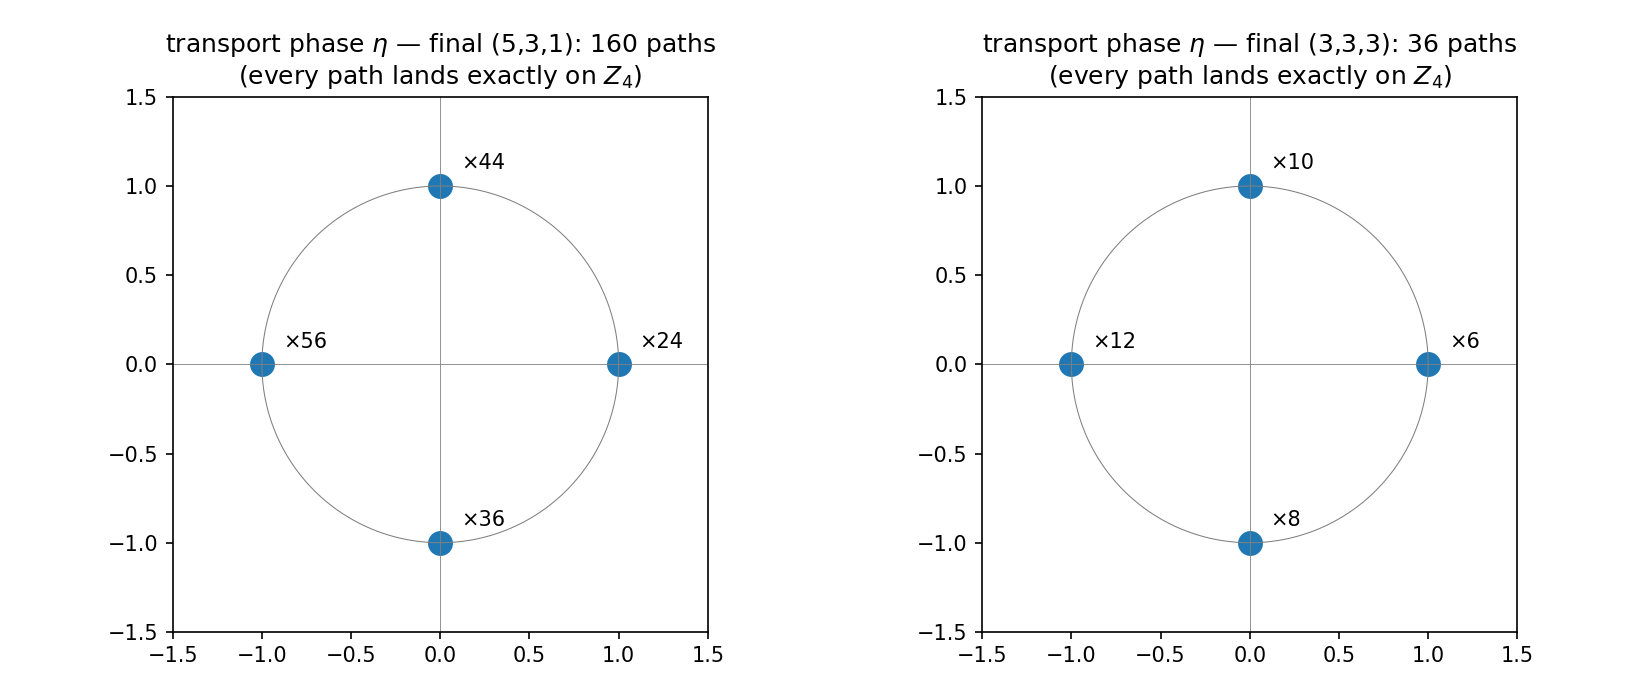
\includegraphics[width=1\linewidth,height=\textheight,keepaspectratio]{paper14_fig1_eta_z4.png}
- \textbf{図2}(\texttt{paper14\_fig2\_convention.png}):
正準規約の2×2分離 --- 対角は無関係(40=40, 160=160)、順序だけが振幅を倍加

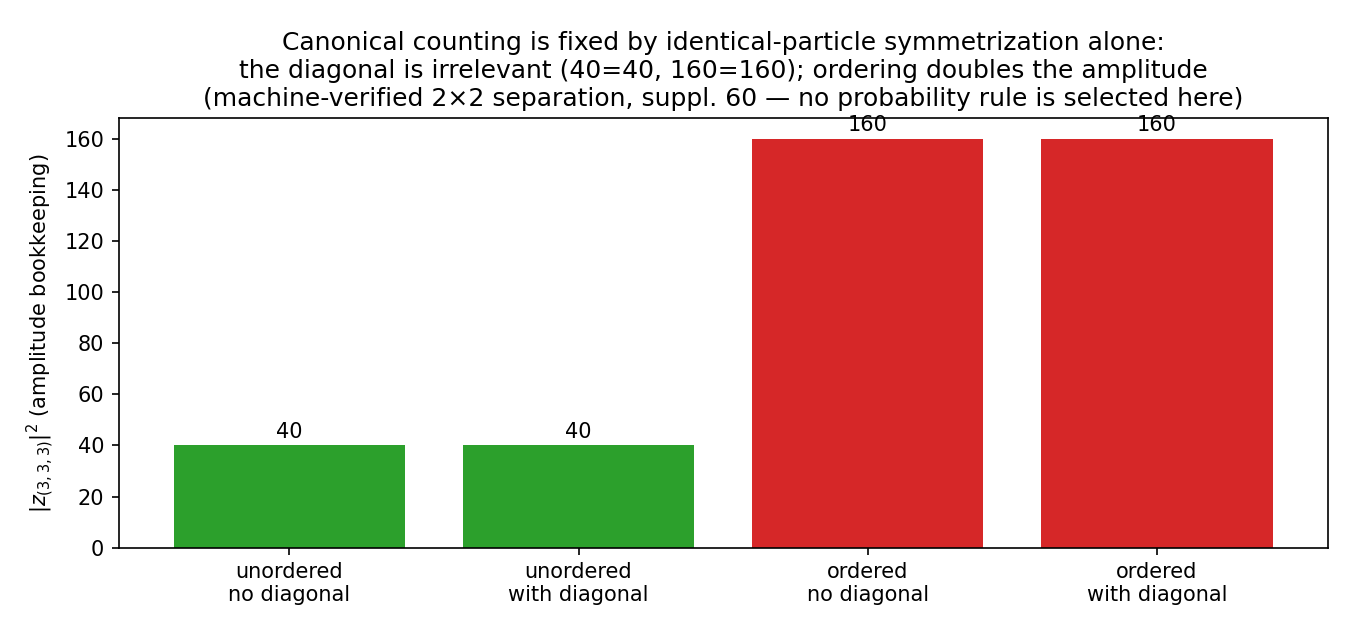
\includegraphics[width=1\linewidth,height=\textheight,keepaspectratio]{paper14_fig2_convention.png}
- \textbf{図3}(\texttt{paper14\_fig3\_holonomy.png}): ビット同定 ---
T1(矢の反転)で不変、片段反転で A↔B、両段で復帰

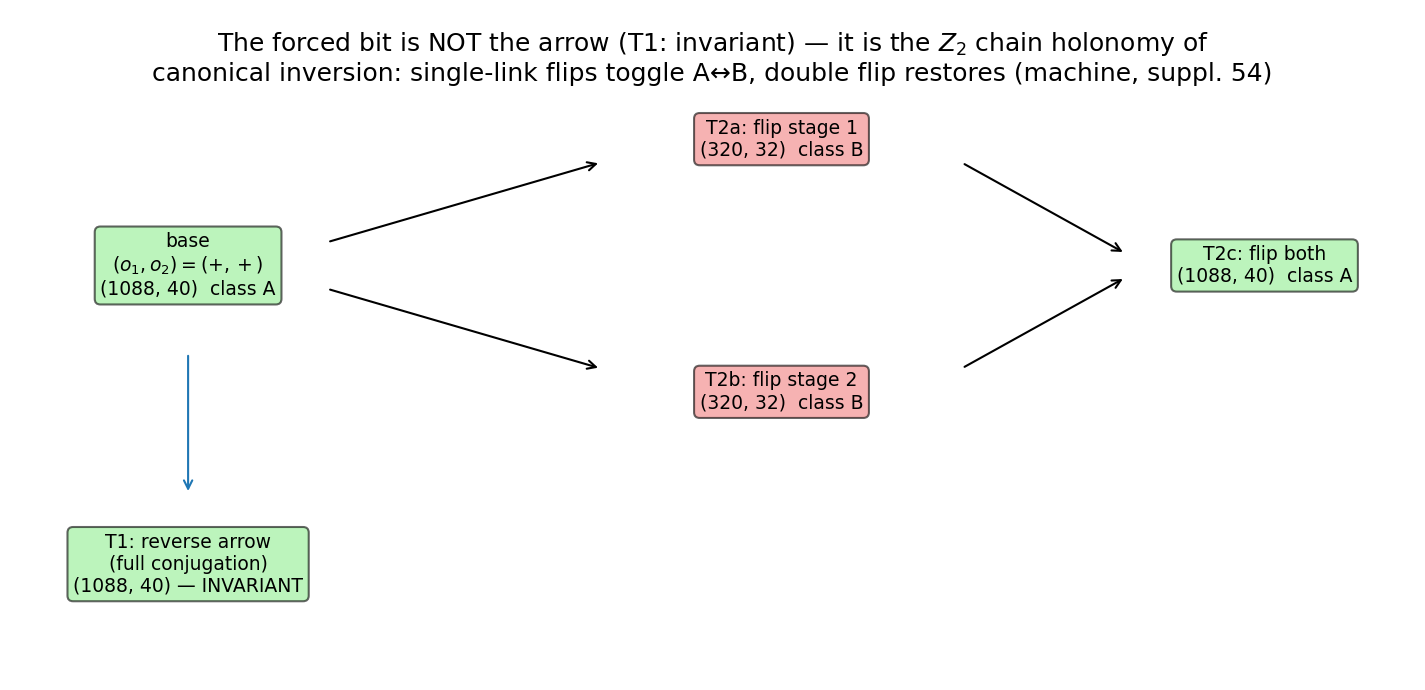
\includegraphics[width=1\linewidth,height=\textheight,keepaspectratio]{paper14_fig3_holonomy.png}

全図は実計算または機械検証済み数値の提示(模式図なし)。

\subsection{付録A:一般輸送代数の補題群(全数検証つき)}\label{ux4ed8ux9332aux4e00ux822cux8f38ux9001ux4ee3ux6570ux306eux88dcux984cux7fa4ux5168ux6570ux691cux8a3cux3064ux304d}

{\def\LTcaptype{none} % do not increment counter
\begin{longtable}[]{@{}
  >{\raggedright\arraybackslash}p{(\linewidth - 4\tabcolsep) * \real{0.3333}}
  >{\raggedright\arraybackslash}p{(\linewidth - 4\tabcolsep) * \real{0.3333}}
  >{\raggedright\arraybackslash}p{(\linewidth - 4\tabcolsep) * \real{0.3333}}@{}}
\toprule\noalign{}
\begin{minipage}[b]{\linewidth}\raggedright
補題
\end{minipage} & \begin{minipage}[b]{\linewidth}\raggedright
内容
\end{minipage} & \begin{minipage}[b]{\linewidth}\raggedright
検証
\end{minipage} \\
\midrule\noalign{}
\endhead
\bottomrule\noalign{}
\endlastfoot
A-1 単軸枝反転 & 単軸の枝反転(cos↔sin)は非零輸送係数に厳密に ±i
を掛け、非零性を保つ & s=9/11/13 全数 \textbf{103,168
反転、零化0・反例0} \\
A-2 単符号支持 & 寄与する交差和は各軸で単符号支持 & 同上 55,267 係数
全数 \\
A-3 電荷様パリティ & \(C\neq0\Rightarrow\varepsilon\)
乗法保存(台のパリティ算術の一行証明)。\textbf{一般補題としては本表が正典であり、論文15
定理8 はその選抜則表現} & 118,944 経路+対照 39.2\%→0 \\
A-4 指数2 & \(|z|^2\) を保つ B₄ 部分群は指数2(192/384) & 全数 \\
A-5 鏡像反転 & 鏡像親への反転で
\(\eta_B/\eta_A=-i(-1)^{\sigma_0}\)(\(\sigma_0\)=第一段娘対の軸0 sin
枝数) & m=2: 10/10、m=3: 384/384(経路集合の一致込み) \\
\end{longtable}
}

これらは\textbf{チャネルや集計規則に依存しない}輸送係数の代数である。チャネル特異的な相殺定理(η²
等分布・A1・B2
等)はチャネル一貫和の測度論的地位に関わるため、本論文には収めない(測度線の管轄
--- §8-1)。

\subsection{付録B:検証一覧}\label{ux4ed8ux9332bux691cux8a3cux4e00ux89a7}

{\def\LTcaptype{none} % do not increment counter
\begin{longtable}[]{@{}
  >{\raggedright\arraybackslash}p{(\linewidth - 6\tabcolsep) * \real{0.2500}}
  >{\raggedright\arraybackslash}p{(\linewidth - 6\tabcolsep) * \real{0.2500}}
  >{\raggedright\arraybackslash}p{(\linewidth - 6\tabcolsep) * \real{0.2500}}
  >{\raggedright\arraybackslash}p{(\linewidth - 6\tabcolsep) * \real{0.2500}}@{}}
\toprule\noalign{}
\begin{minipage}[b]{\linewidth}\raggedright
主張
\end{minipage} & \begin{minipage}[b]{\linewidth}\raggedright
ラベル(①構成により真/②定理+確認/③落ちえた検査)
\end{minipage} & \begin{minipage}[b]{\linewidth}\raggedright
検証
\end{minipage} & \begin{minipage}[b]{\linewidth}\raggedright
方式
\end{minipage} \\
\midrule\noalign{}
\endhead
\bottomrule\noalign{}
\endlastfoot
命題1′ 恒等式・奇性 & \textbf{②(3行証明あり)} & 6561セル & 範囲内確認 \\
定理2 マーキング(列挙・推移性) & ③ & 384元の移送積表の重複除去 & 全数 \\
定理2(ii) 共有読み & ③ & B₄ 全384元の不変性 & 全数 \\
定理3 Z₄ 量子化 & ③ & s=9/11/13 全経路 & 全数 \\
定理4 T1/T2 & ③ & 向き群 Z₂×Z₂=4元 & 全数(向き群)+標本 \\
定理4 範囲限定の付記(W′) & ③ & s=9 両セクター & 全数 \\
定理5 2×2分離(順序×対角) & ③ & 4規約×2チャネル & 全数 \\
補題 A-1/A-2 & ③(一般 s 証明はキュー) & 103,168/55,267 & 全数 \\
補題 A-5 & ②(3行算術=証明) & 394経路 & 全数確認 \\
\end{longtable}
}

\begin{center}\rule{0.5\linewidth}{0.5pt}\end{center}

\textbf{謝辞・履歴}: 検証は Claude Code(ローカル機械検証)と
claude.ai(独立検算)の二者独立検算プロトコルによる。素材:補遺49〜54・56〜60・70・71・80(補題A-5
の導出=claude.ai、検証=Claude
Code)・81(2026-06-12)。v0.2:第1回査読(中改訂)\#1〜\#5
反映。v1.0:第2回査読(採録・軽微条件付き)R1〜R6 反映 ---
命題1′の証明転記(claude.ai による3行証明)・ラベル列・W′
検証スクリプト名・セクター用語注記・第1回推奨の一括処理。

物理的同一視は行わない。

\end{document}
